% generated by docs/audit/make_tables.py -- do not edit by hand
\begin{figure}[p]\centering
\begin{minipage}[t]{0.86\textwidth}\centering
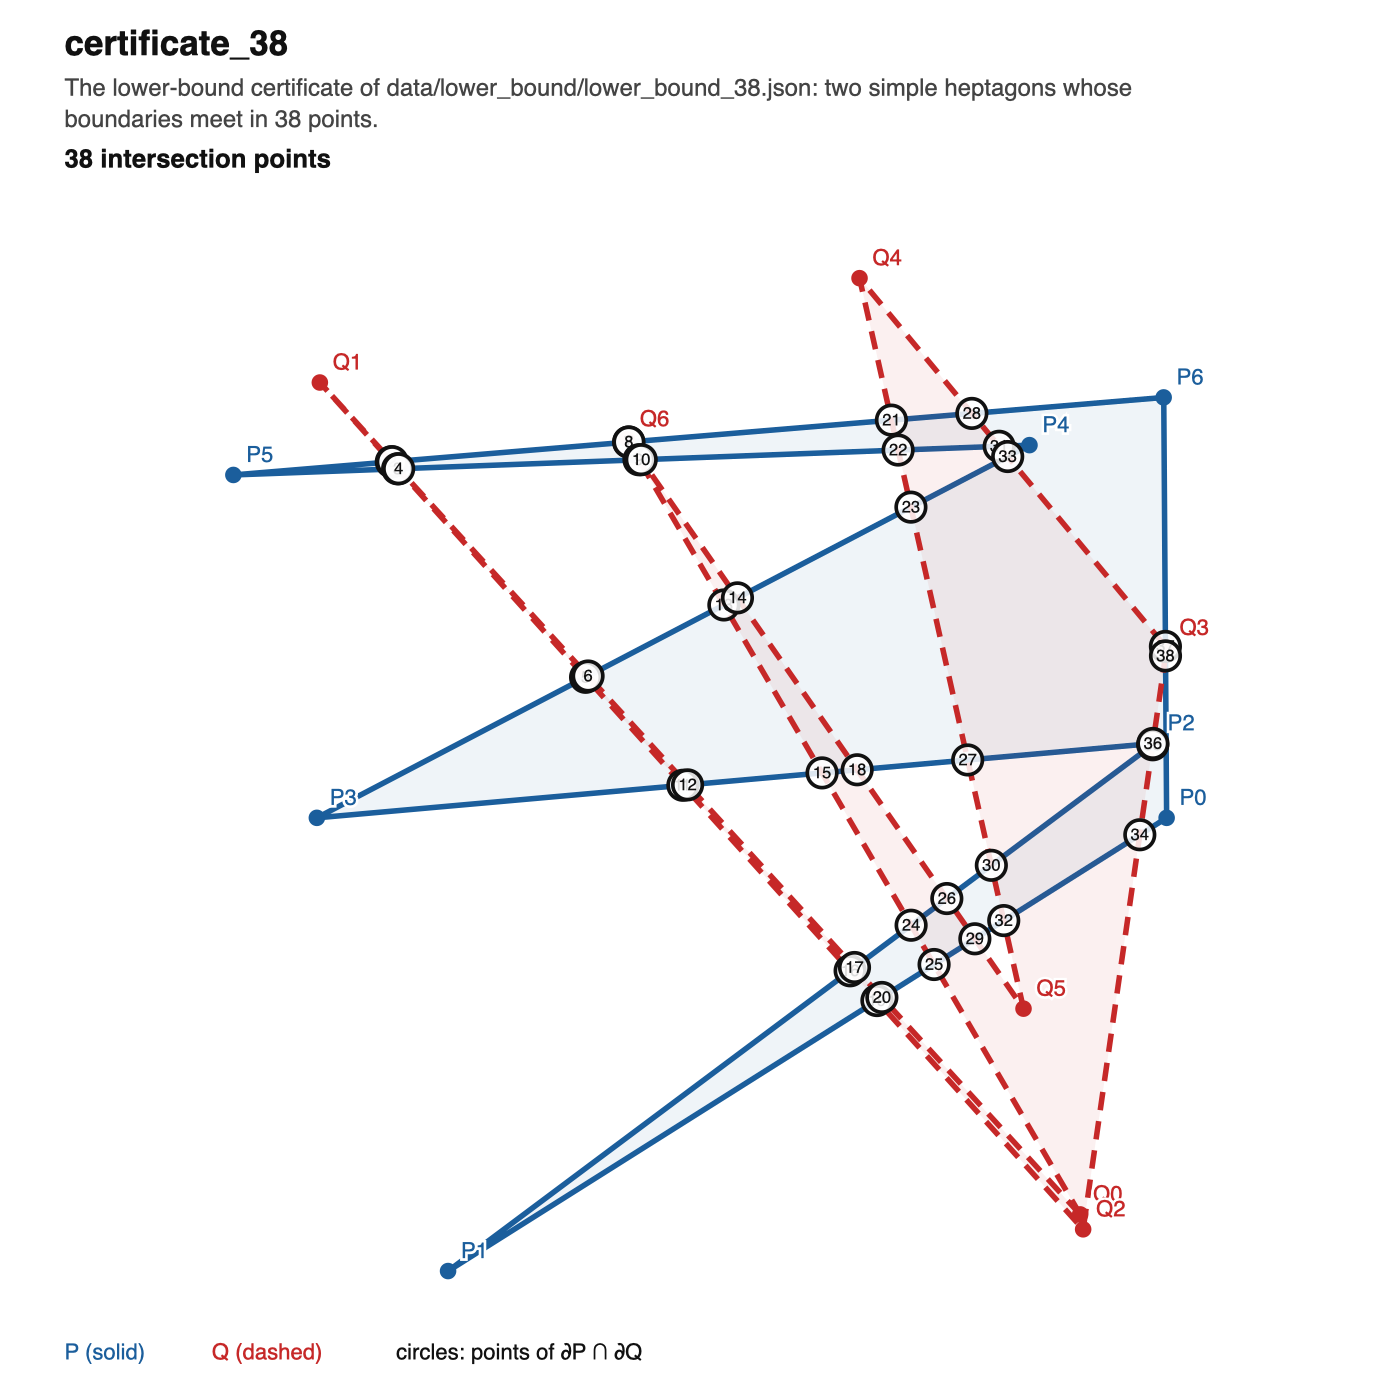
\includegraphics[width=\linewidth]{out/png/certificate_38.svg.png}
\par\smallskip{\footnotesize\texttt{certificate\_38}\\[1pt]computed count: \textbf{38}}
\end{minipage}
\caption{The lower-bound certificate. Every point of $\partial P\cap\partial Q$ is circled and numbered; there are \textbf{38}. This is the same configuration the Lean proof uses as its witness, read from the same JSON file.}
\end{figure}
\begin{figure}[p]\centering
\begin{minipage}[t]{0.45\textwidth}\centering
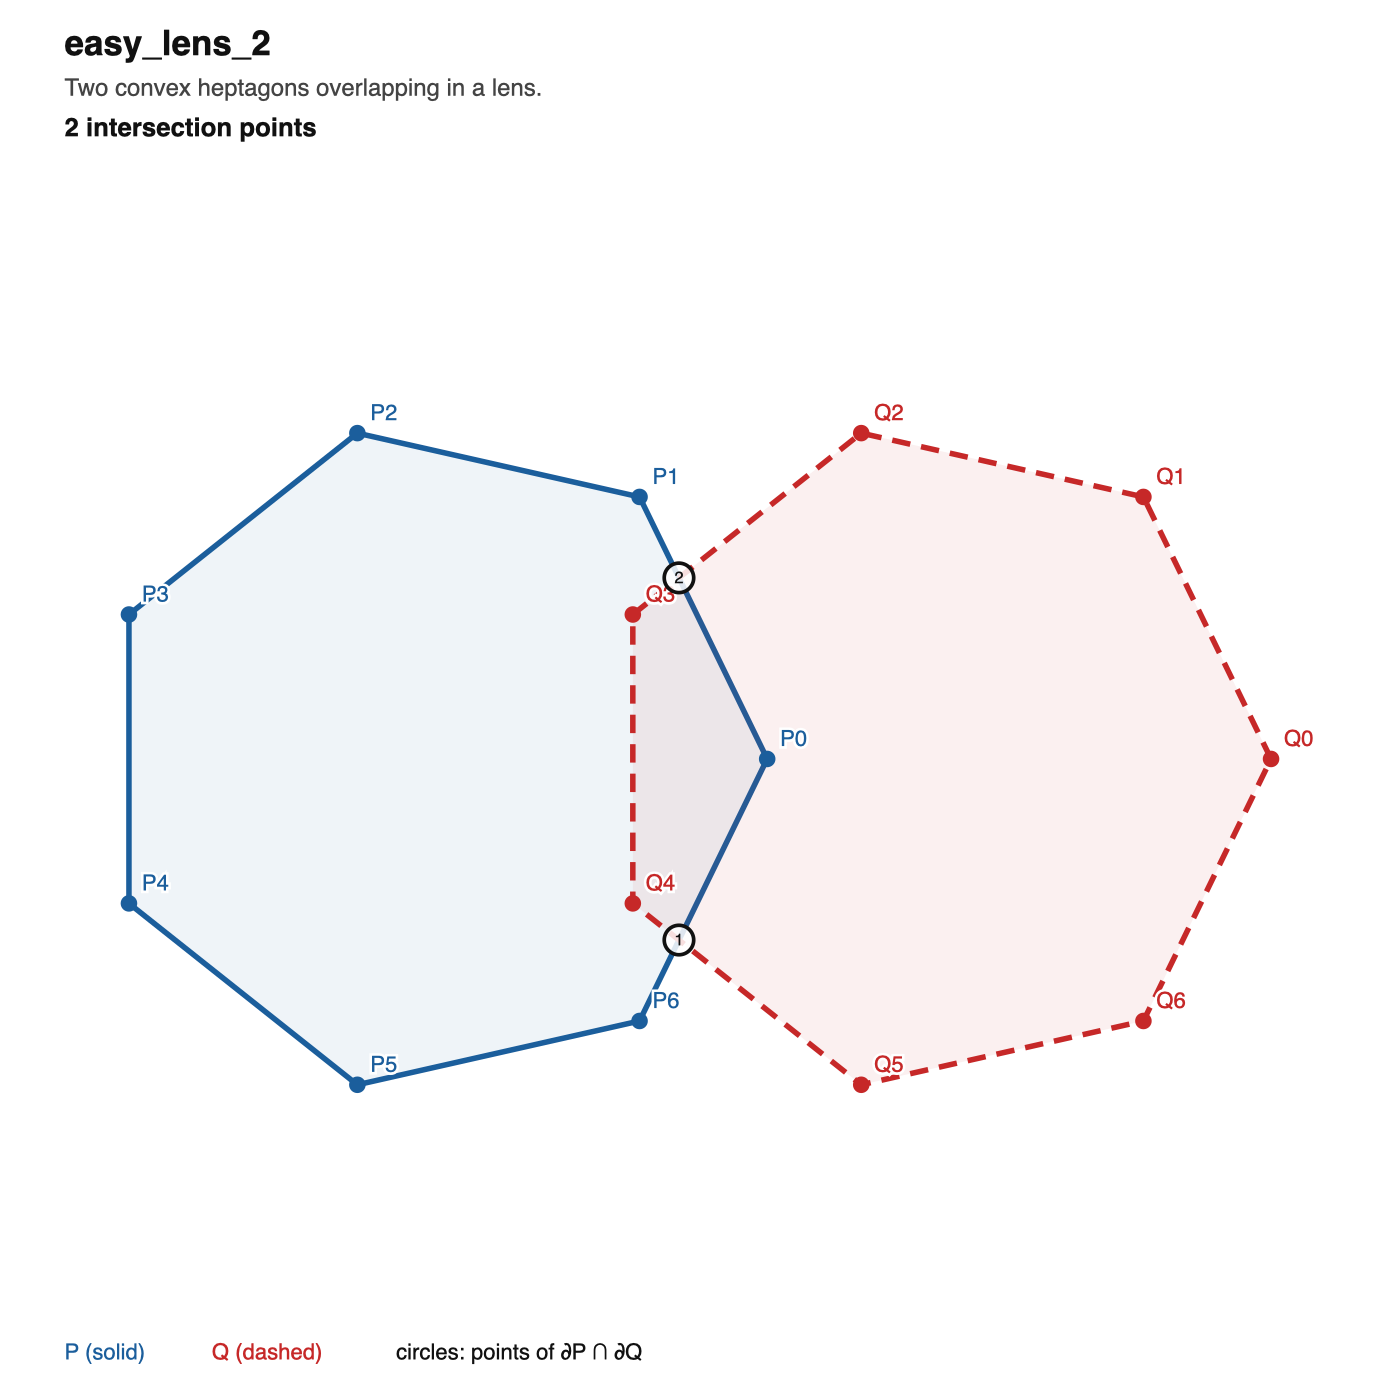
\includegraphics[width=\linewidth]{out/png/easy_lens_2.svg.png}
\par\smallskip{\footnotesize\texttt{easy\_lens\_2}\\[1pt]computed count: \textbf{2}}
\end{minipage}
\hfill
\begin{minipage}[t]{0.45\textwidth}\centering
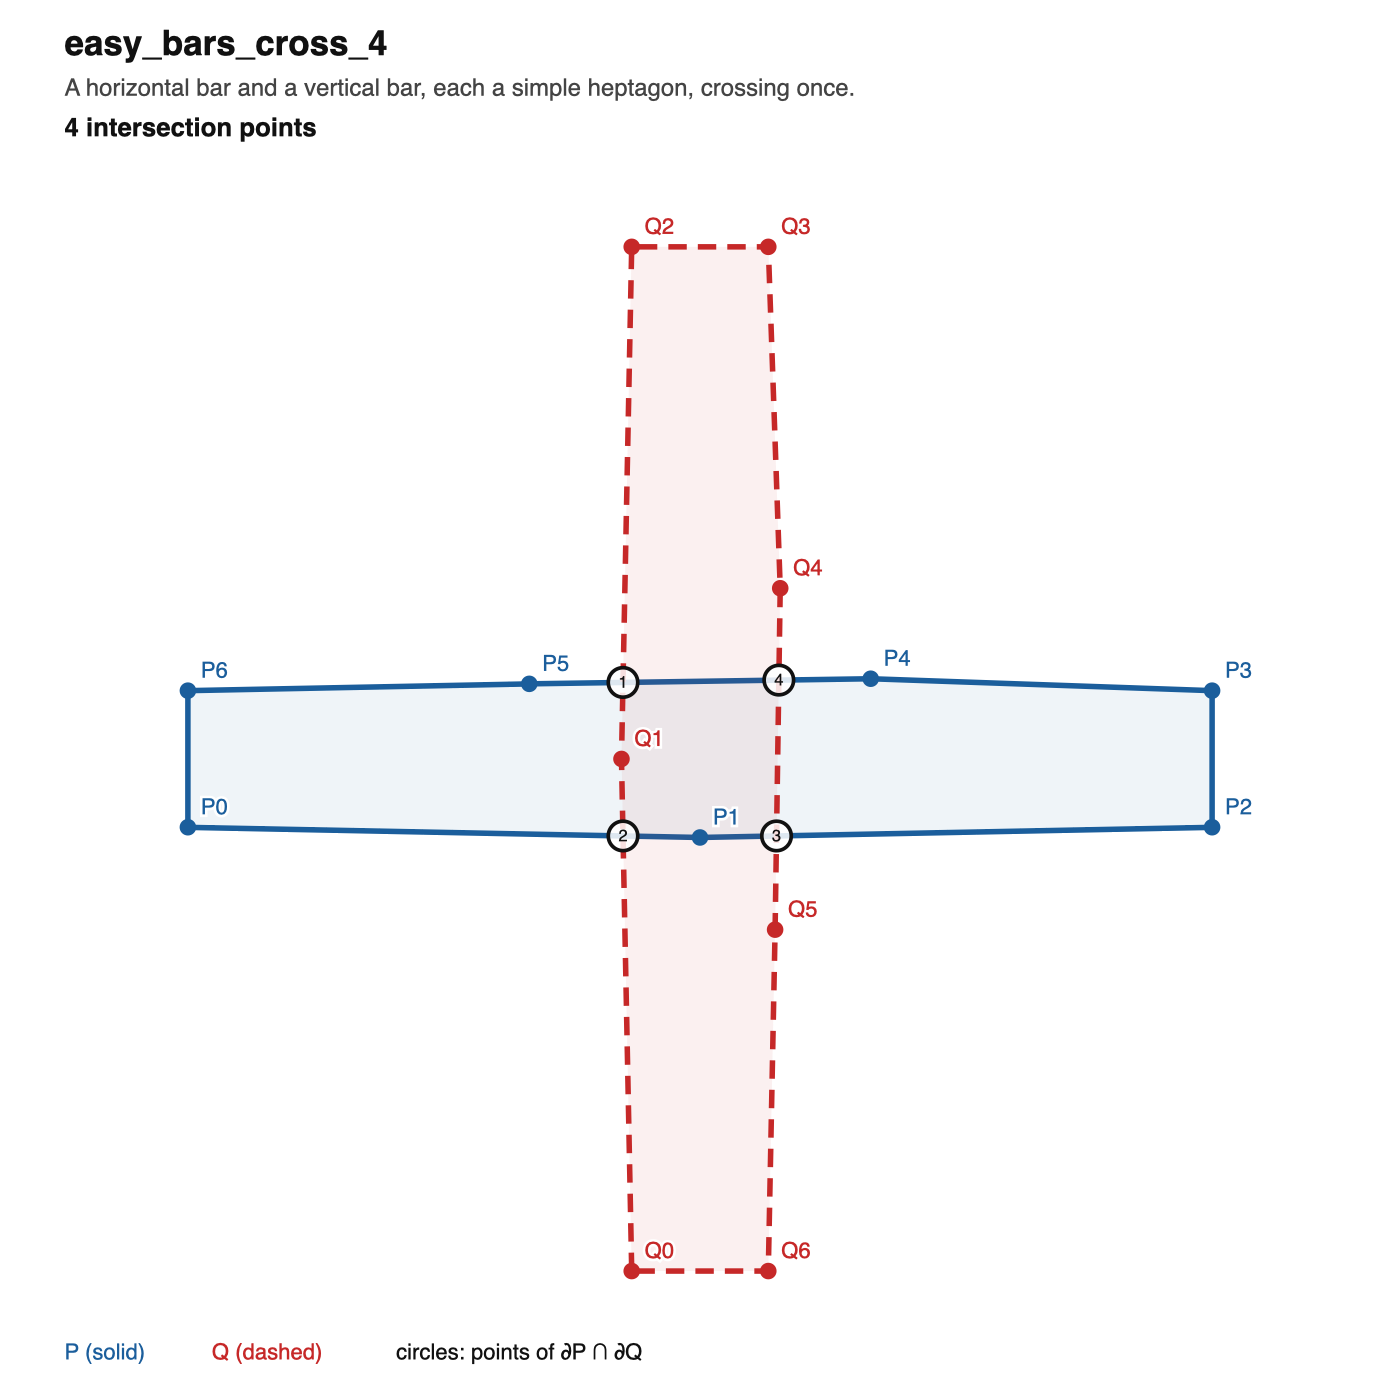
\includegraphics[width=\linewidth]{out/png/easy_bars_cross_4.svg.png}
\par\smallskip{\footnotesize\texttt{easy\_bars\_cross\_4}\\[1pt]computed count: \textbf{4}}
\end{minipage}
\par\bigskip
\begin{minipage}[t]{0.45\textwidth}\centering
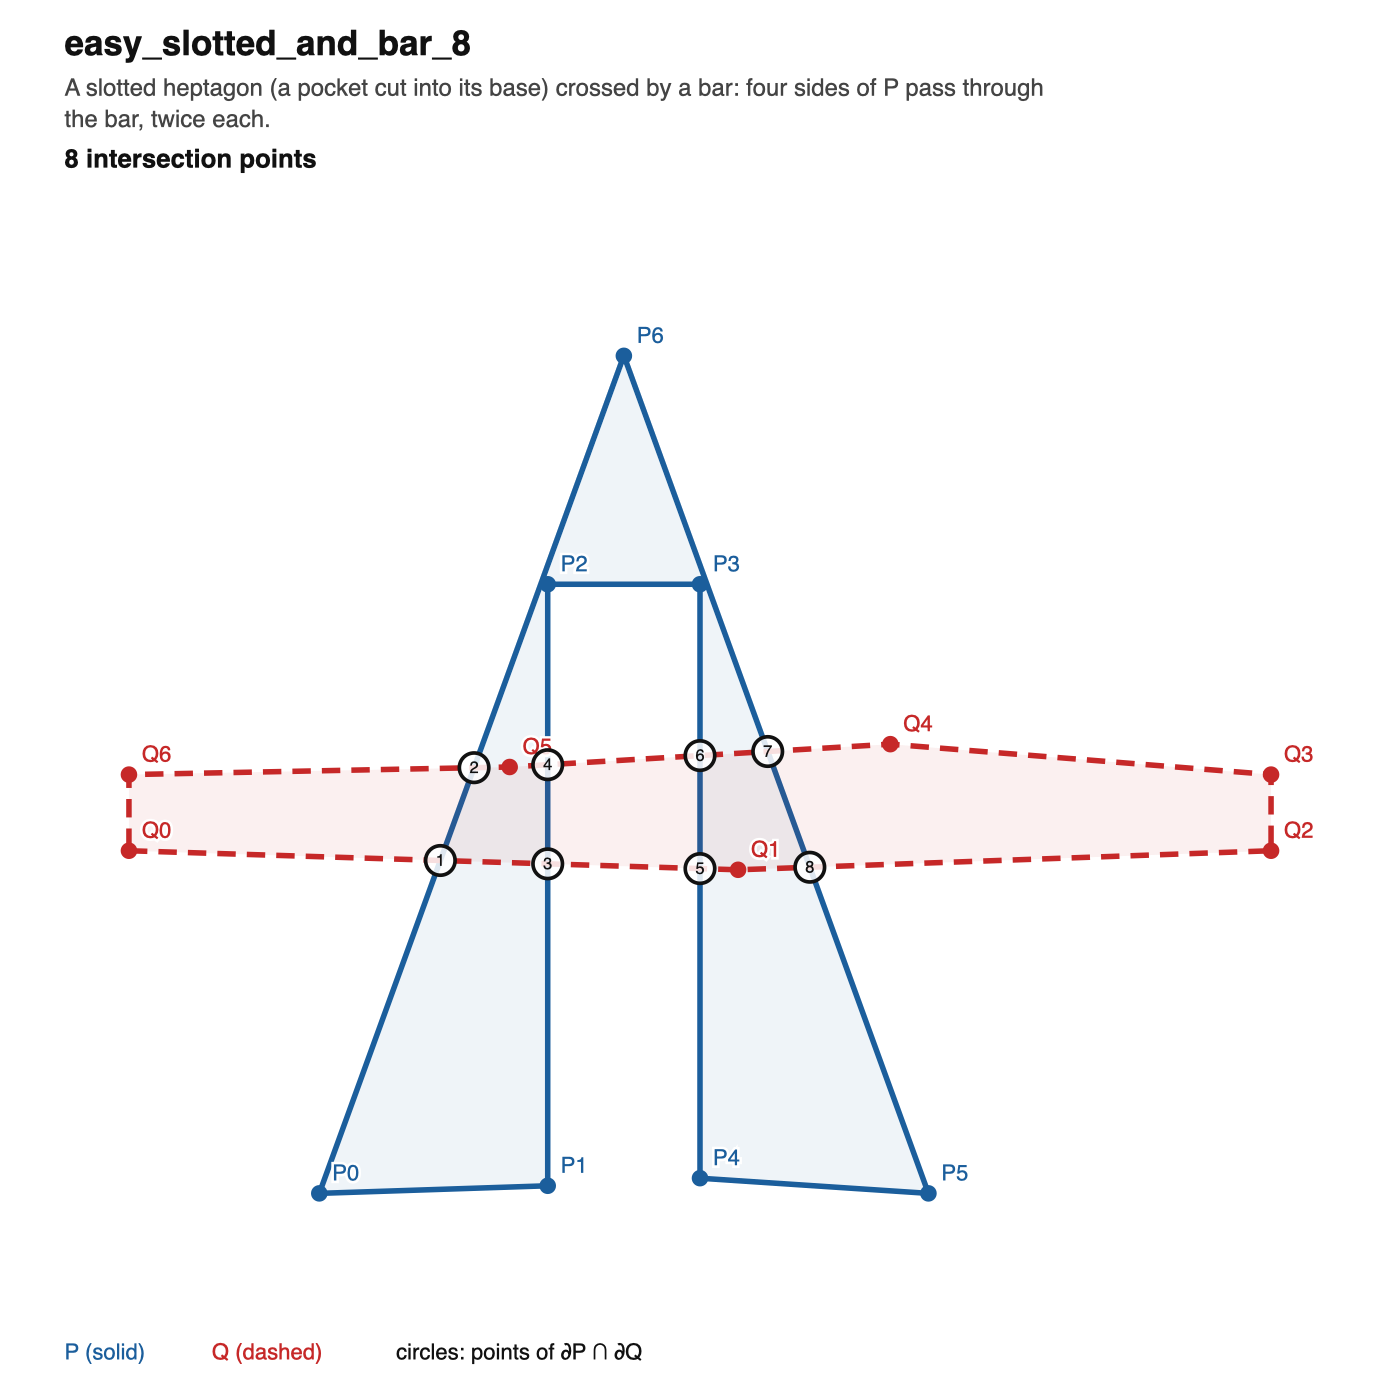
\includegraphics[width=\linewidth]{out/png/easy_slotted_and_bar_8.svg.png}
\par\smallskip{\footnotesize\texttt{easy\_slotted\_and\_bar\_8}\\[1pt]computed count: \textbf{8}}
\end{minipage}
\hfill
\begin{minipage}[t]{0.45\textwidth}\centering
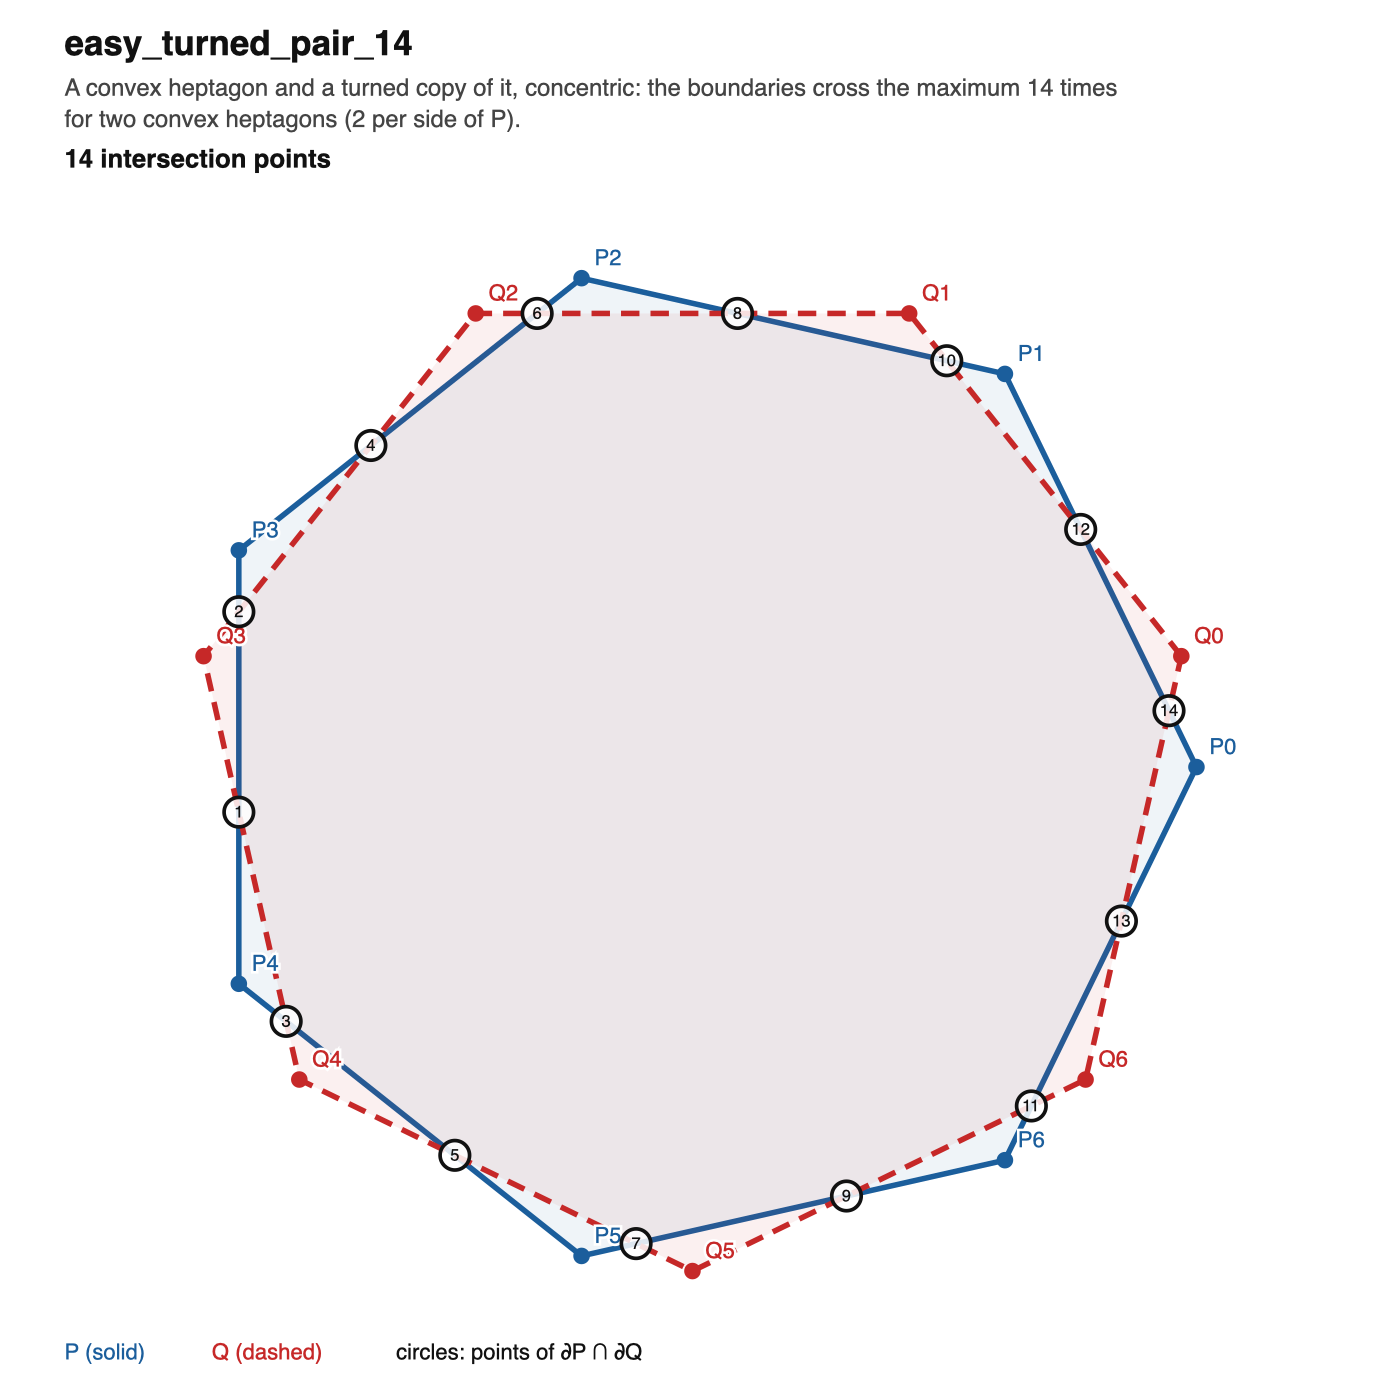
\includegraphics[width=\linewidth]{out/png/easy_turned_pair_14.svg.png}
\par\smallskip{\footnotesize\texttt{easy\_turned\_pair\_14}\\[1pt]computed count: \textbf{14}}
\end{minipage}
\par\bigskip
\caption{Sanity checks with answers you can see at a glance.}
\end{figure}
\begin{figure}[p]\centering
\begin{minipage}[t]{0.45\textwidth}\centering
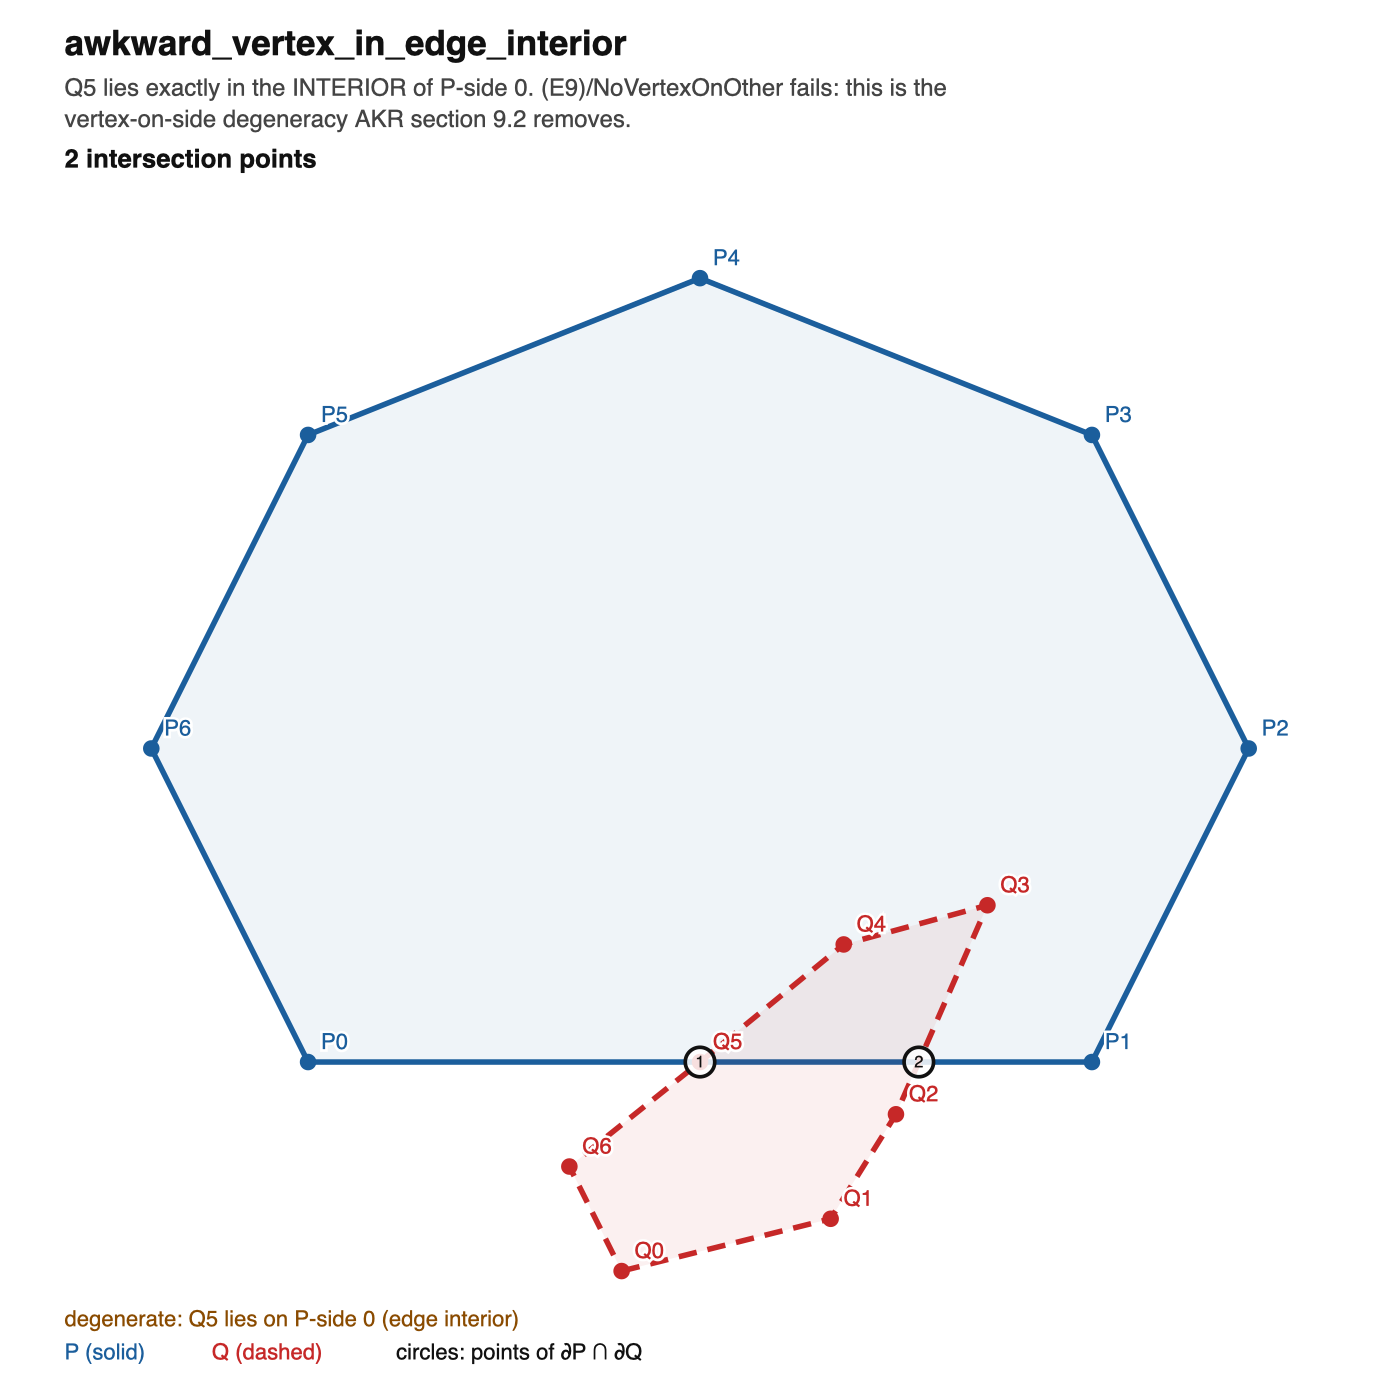
\includegraphics[width=\linewidth]{out/png/awkward_vertex_in_edge_interior.svg.png}
\par\smallskip{\footnotesize\texttt{awkward\_vertex\_in\_edge\_interior}\\[1pt]computed count: \textbf{2}}
\end{minipage}
\hfill
\begin{minipage}[t]{0.45\textwidth}\centering
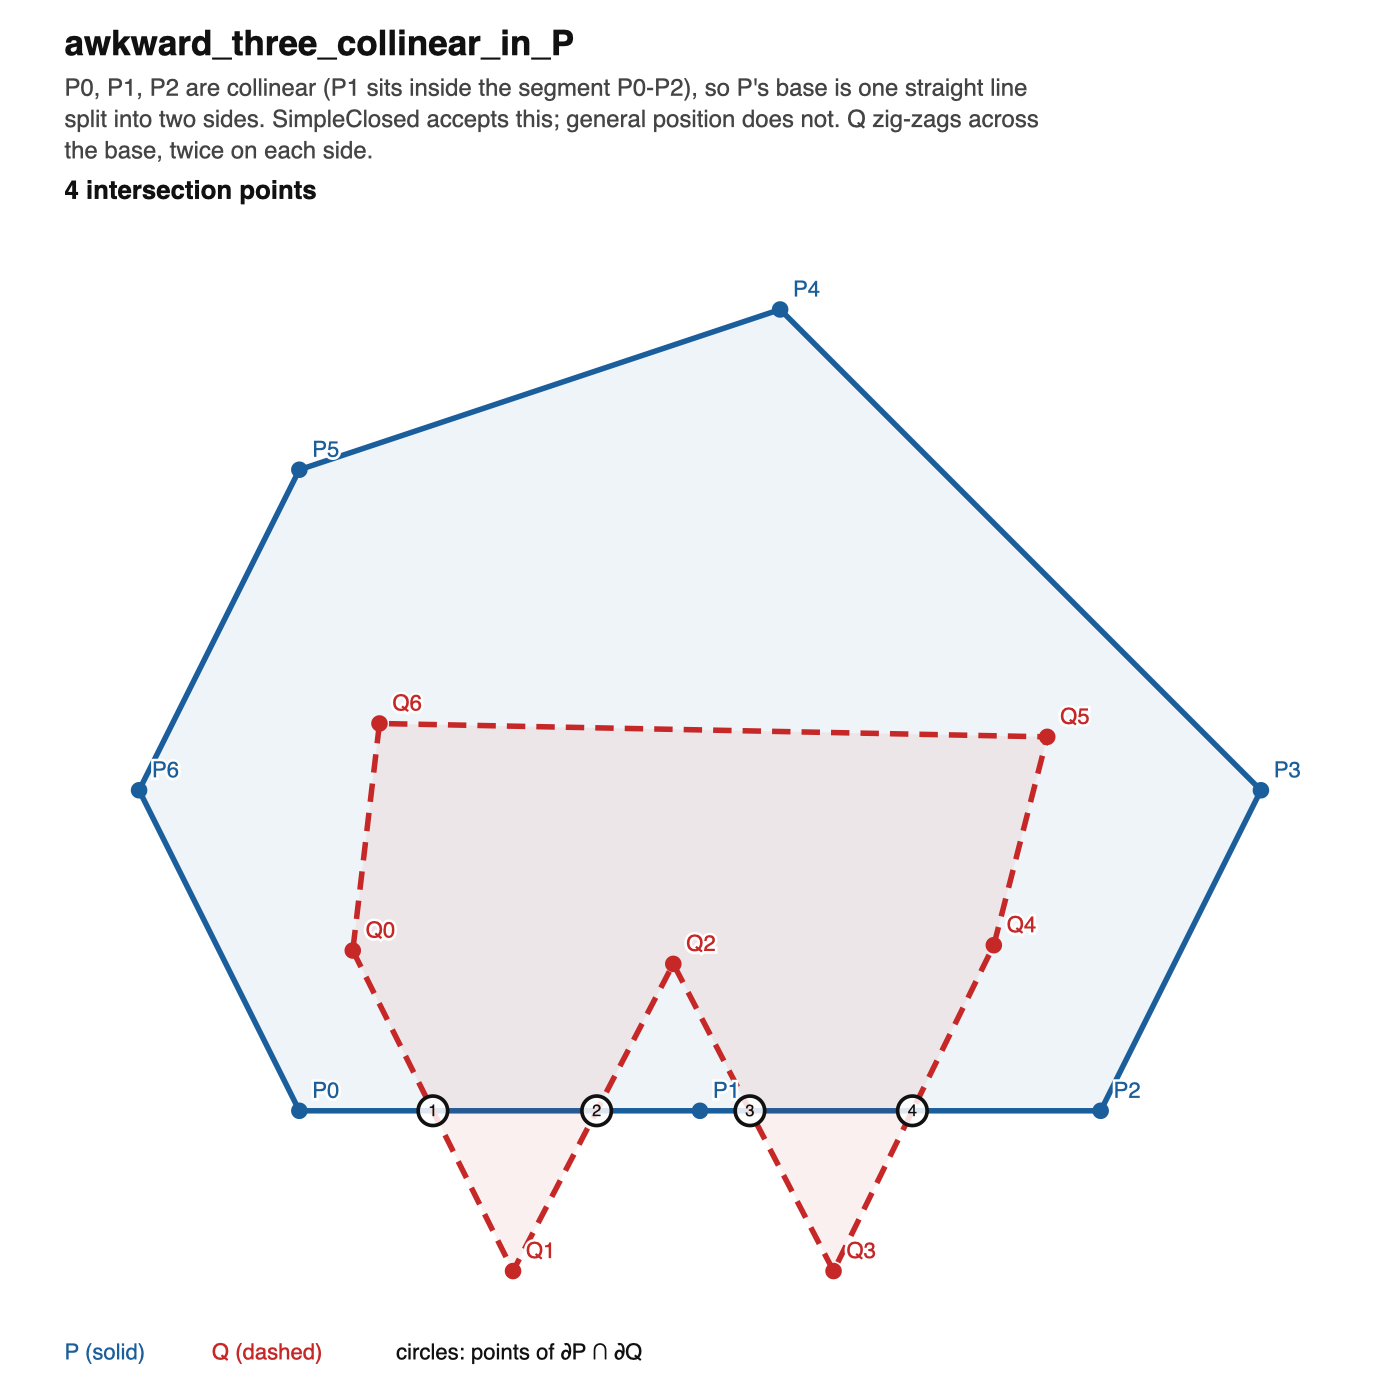
\includegraphics[width=\linewidth]{out/png/awkward_three_collinear_in_P.svg.png}
\par\smallskip{\footnotesize\texttt{awkward\_three\_collinear\_in\_P}\\[1pt]computed count: \textbf{4}}
\end{minipage}
\par\bigskip
\begin{minipage}[t]{0.45\textwidth}\centering
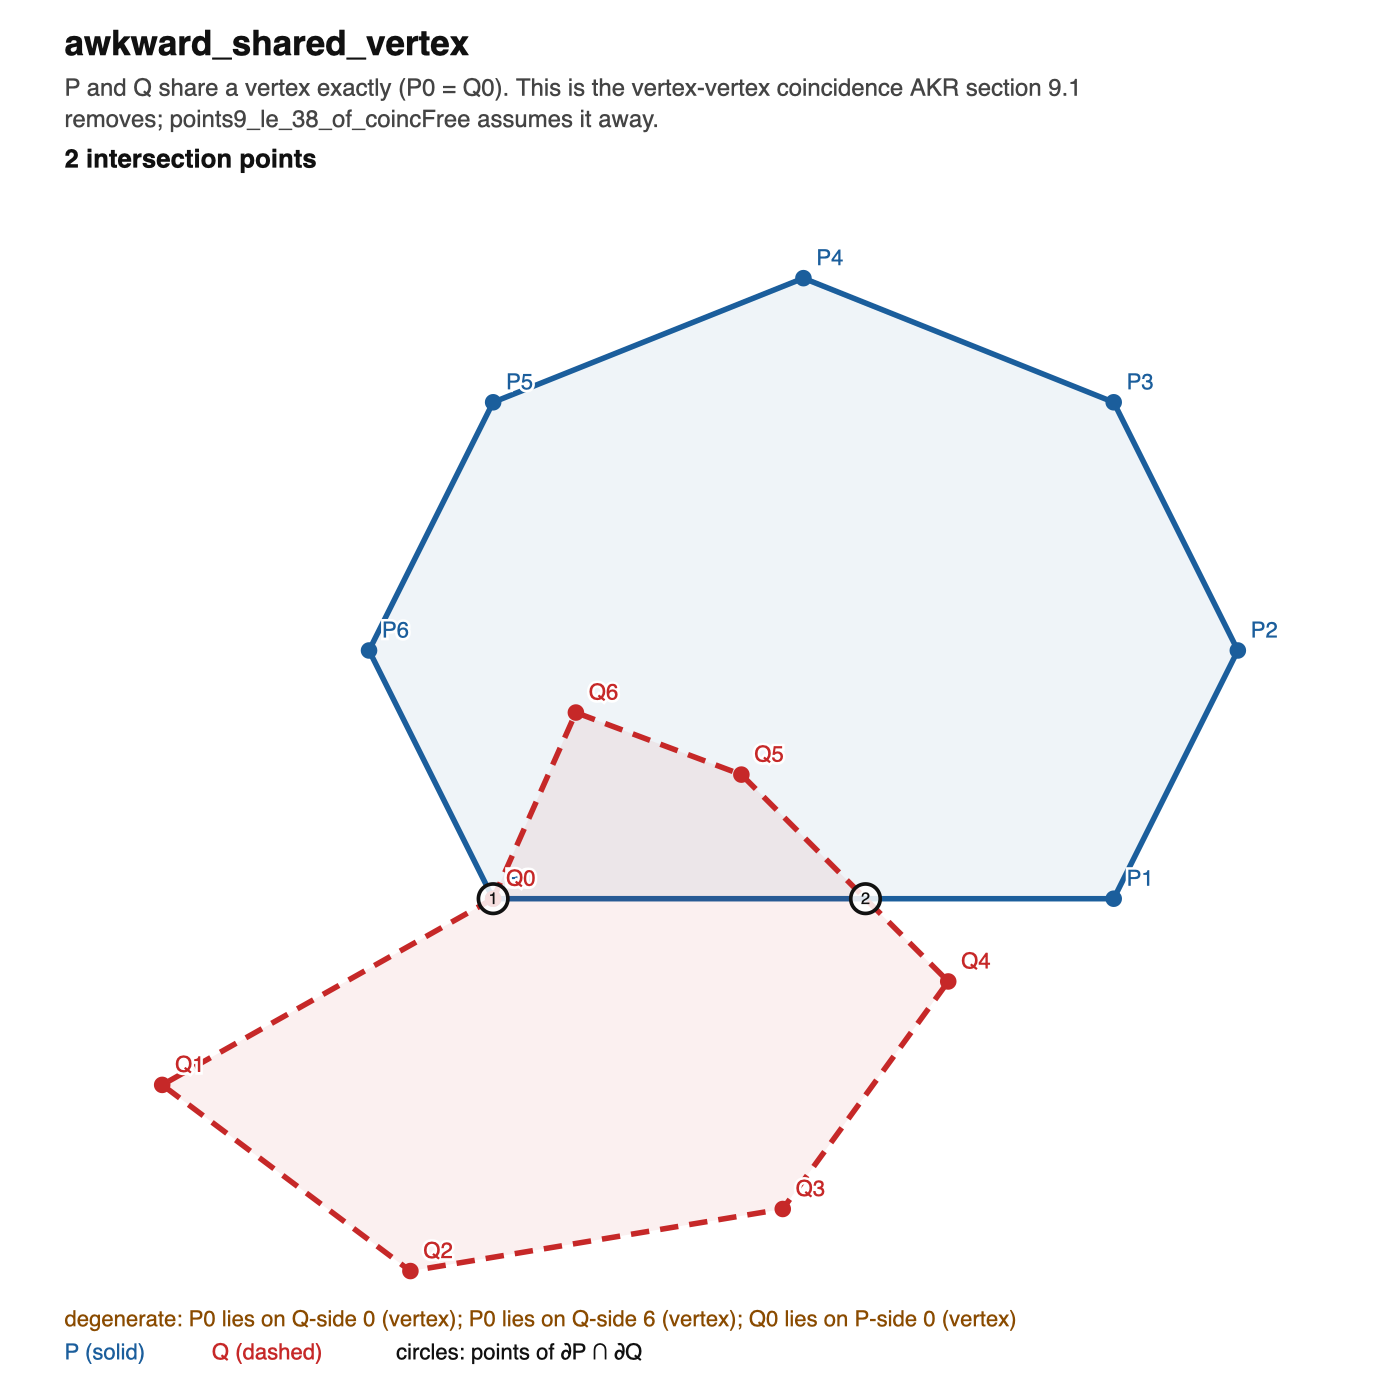
\includegraphics[width=\linewidth]{out/png/awkward_shared_vertex.svg.png}
\par\smallskip{\footnotesize\texttt{awkward\_shared\_vertex}\\[1pt]computed count: \textbf{2}}
\end{minipage}
\hfill
\begin{minipage}[t]{0.45\textwidth}\centering
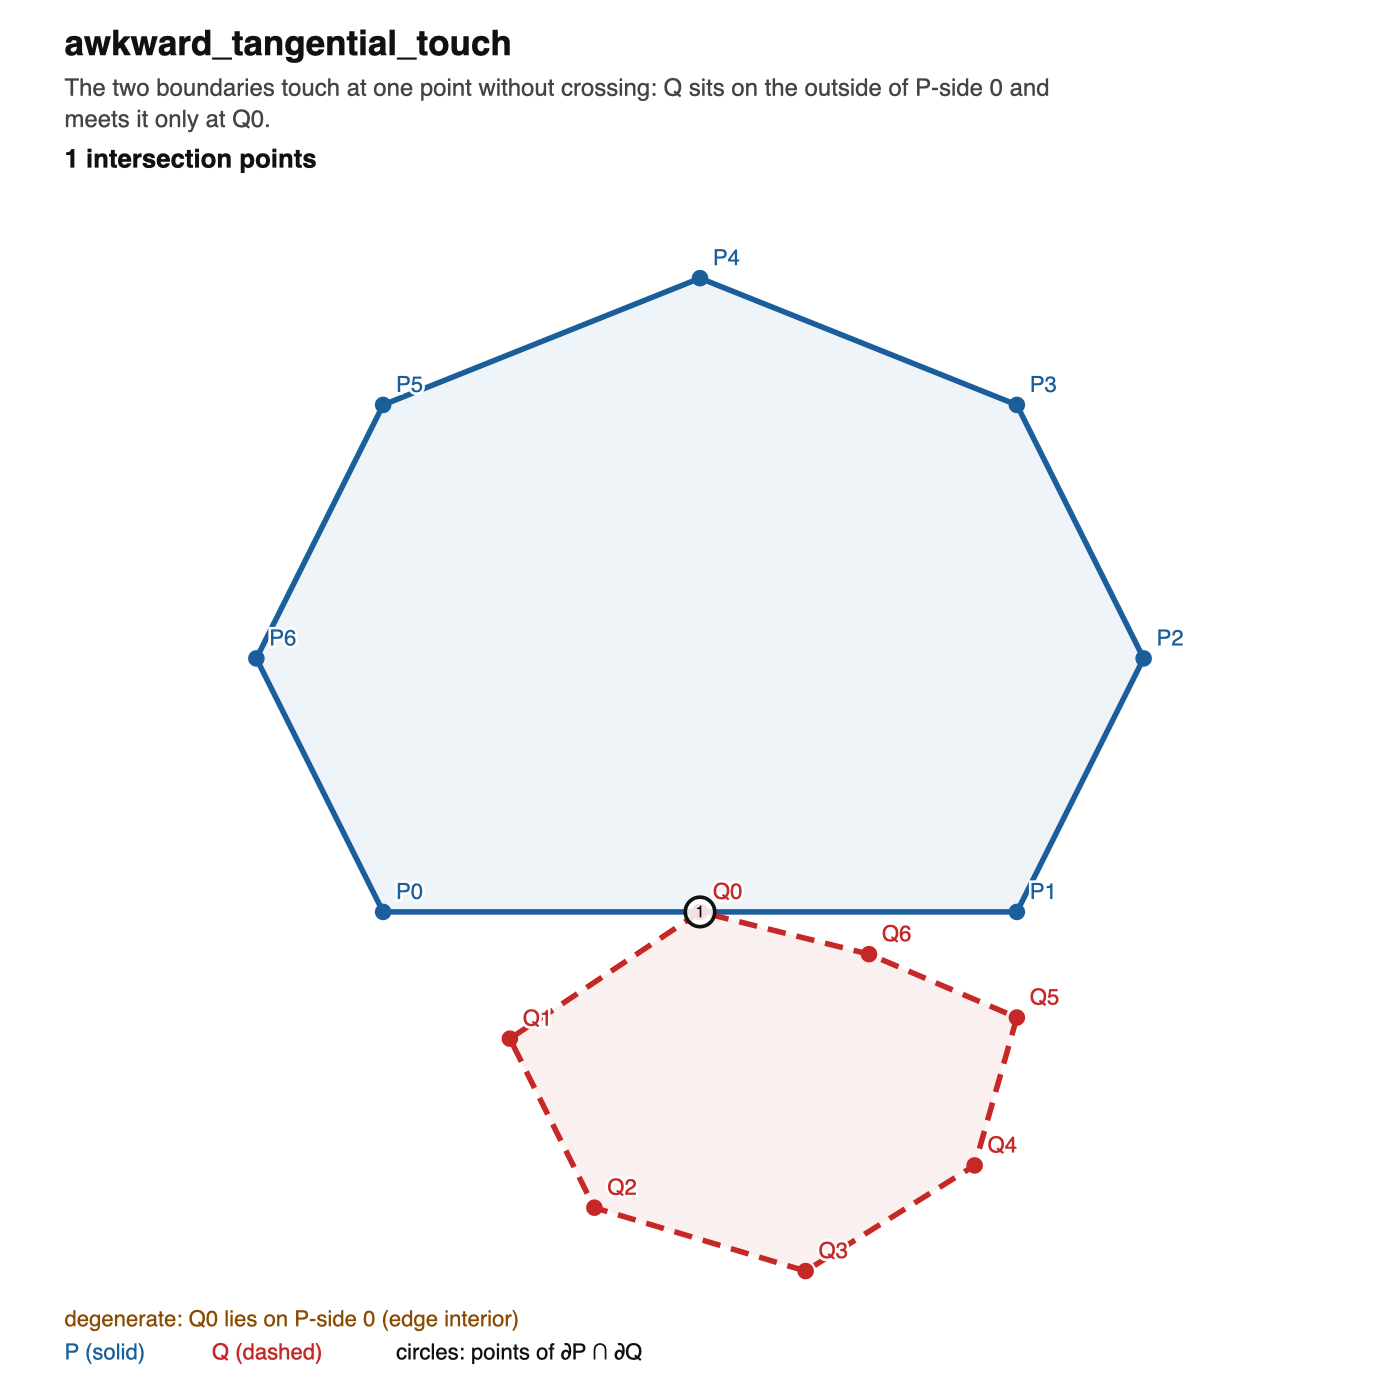
\includegraphics[width=\linewidth]{out/png/awkward_tangential_touch.svg.png}
\par\smallskip{\footnotesize\texttt{awkward\_tangential\_touch}\\[1pt]computed count: \textbf{1}}
\end{minipage}
\par\bigskip
\caption{Degeneracies that the theorem's hypotheses \emph{allow}, plus the one they exclude (\texttt{awkward\_shared\_vertex}).}
\end{figure}
\begin{figure}[p]\centering
\begin{minipage}[t]{0.45\textwidth}\centering
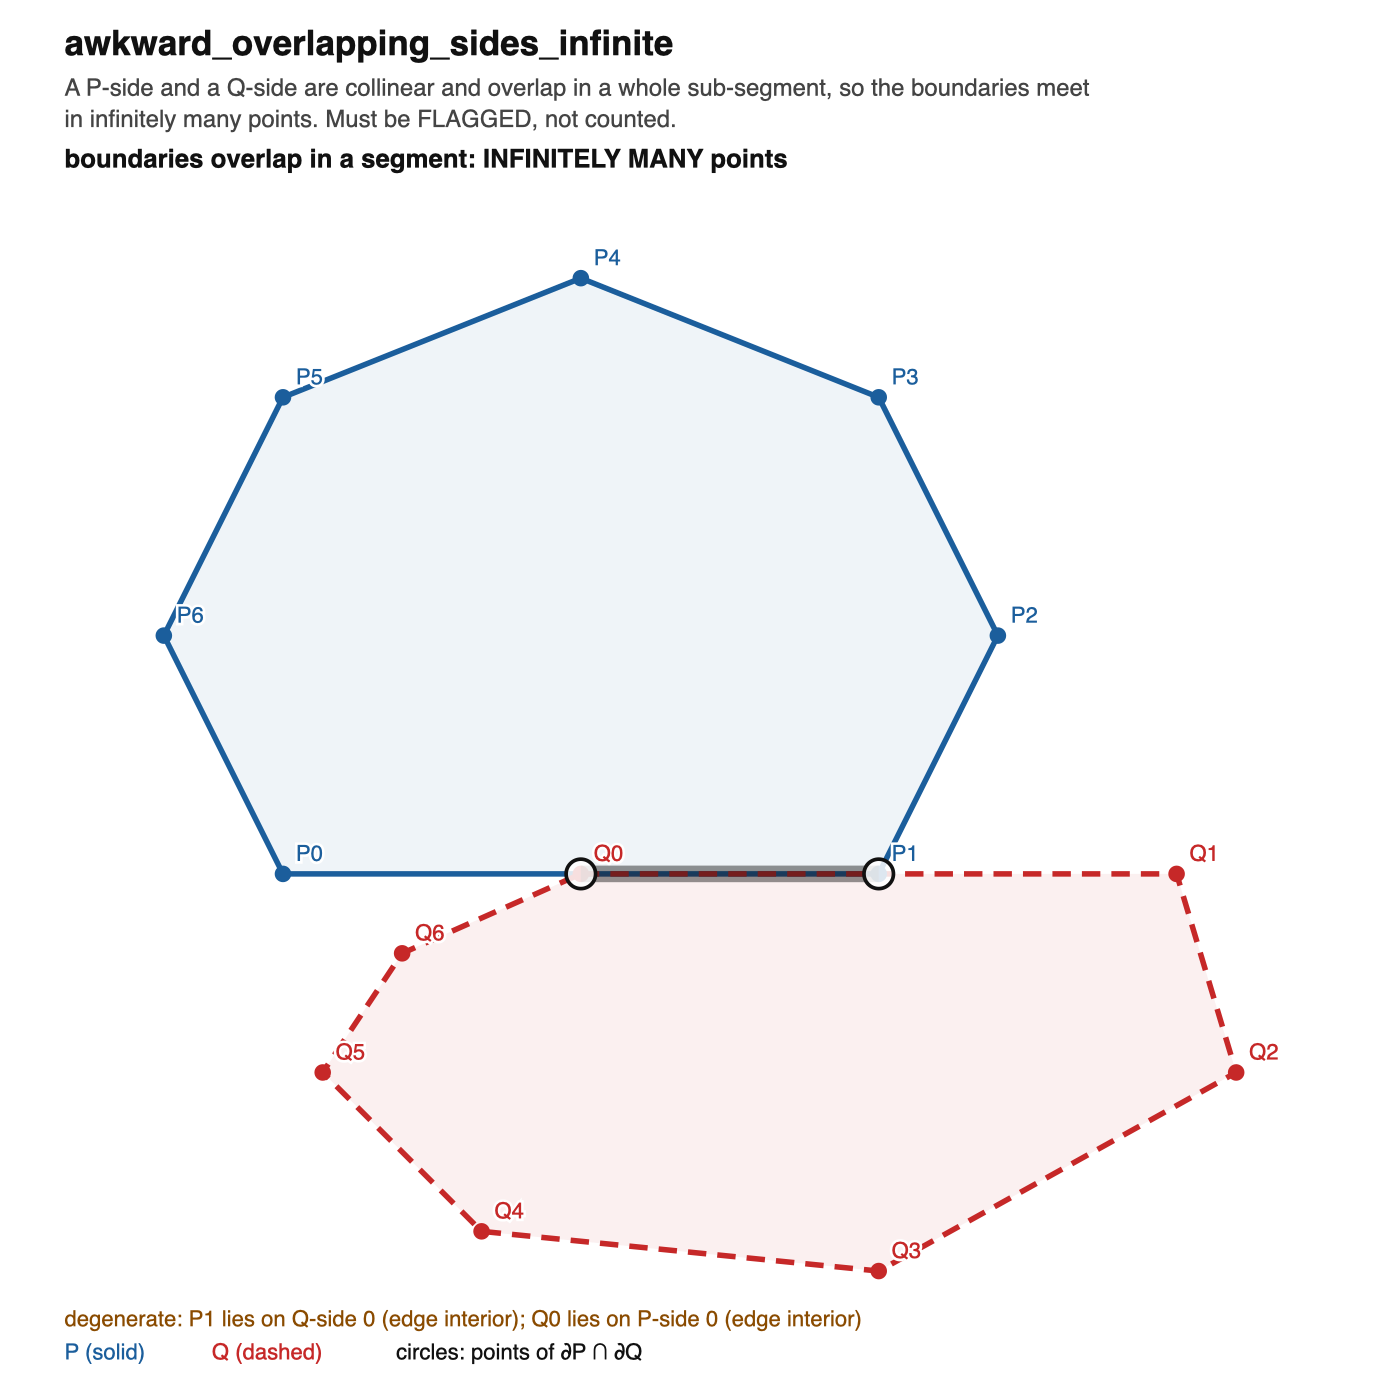
\includegraphics[width=\linewidth]{out/png/awkward_overlapping_sides_infinite.svg.png}
\par\smallskip{\footnotesize\texttt{awkward\_overlapping\_sides\_infinite}\\[1pt]computed count: \textbf{\textsc{infinite}}}
\end{minipage}
\hfill
\caption{The honest failure mode: two sides overlap in a whole sub-segment, so the intersection is genuinely infinite. It is flagged, not miscounted.}
\end{figure}
